
\section{TJ-Monopix1 characterization}
    \subsection{Threshold and noise: figure of merit for pixel detectors}
        %python3 -i calibration/scurve_tot_histo.py -f calibration/calibration_data/20220506 -i 1 100 questo script crea i file di output contenenti i gli istogrammi del tot e della s curve
        %python3 -i calibration/tot_charge_plotting.py -f calibration/calibration_data/20220506 per fare il plot della s curve e relativi residui 
        %python3 -i calibration/tot_histo2d.py -f calibration/calibration_data/PMOS/20220506 per fare l'istogramma 2d del tot
 
        The threshold has to be high enough to cut the noise, but also low enough to mantain a high signal efficiency, and 
        For low enough threshold and/or enough pixels firing at the same time, this positive feedback can set off a chain reaction causing all pixels to fire. For a given instantaneous hit occupancy (fraction of pixels firing atthe same time due to an external stimulus), there will be a minimum stable threshold.
        For this reason the signal to threshold ratio, rather than the signal to noise ratio, can be considered as the figure of merit for pixel detectors.


        la soglia è collegato al rumore, nel senso che: supponiamo di volere un occupancy di 10-4
        allora sceglierò la soglia in base a questo. (plot su quaderno)
        Da questo conto trovo la minima soglia mettibile\\
        In realtà quello che faccio è mettere una soglia un po' più grande perchè il rate di rumore
        dipende da molti fattori quali la temperatura, l anneling ecc, e non voglio che cambiando leggermente
        uno di questi parametri vedo alzarsi molto il rate di rumore. In realtà non è solo il
        rumore sensibile a diversi fattori, ma anche la soglia: ad esempio la cosa classica è
        la variabilità della soglia da pixel a pixel.\\
        In questo modo rumore e soglia diventano parenti.\\

        The front end noise does set a lower bound to the threshold, but does not determine how far above this lower bound is the minimum stable threshold. Assuming a noise occupancy of 10meno4 is acceptable, this corresponds to the Gaussian 1-sided tail fraction for 3.7sigma . Inverting the question, for a 500 e minimum threshold, the noise must be less than 500/3.7=135 e equivalent input charge. But this is just an upper bound. How far below this bound the noise needs to be depends on how the threshold varies with time and how frompixel to pixel.

        Questo implica tra le altre cose che voglio poter assegnare delle soglie diverse
        a diversi pixel. Non fare trimming sulla soglia è uno dei problemi che si sono sempre incontrati: a casusa dei mismatch dei transistor
        le soglie efficaci pixel per pixel cambiano tanto.


        ASSEGNAZIONE DELLE SOGLIE IN TJ MONOPIX E ARAVDIA.
        Drawback è dare spazio per registri e quantaltro. Ad esempio per Monopix1 la soglia è locale, poi 3 bit vengono allocati per trimming sul singolo pixel.
        Arcadia invece 
        Questo lascia però ancora aperto il problema temporale delle variazioni del rumore:
        problema per cui diventano necessarie le misure dei sensori dopo l'irraggiamento.\\

        La larghezza della s curve è il noise se assumi che il noise è gaussiano


        Il trimming della soglia avviene con dei DAC: la dispersione della soglia dopo al tuning e dovuta al dac è: 
        \begin{equation}
            \sigma_{THR, tuned} = \frac{\sigma_{THR}}{2^{n bit}}
        \end{equation}
        dove il numero di bit cambia varia tra 3-7 tipicamente. Monopix è 7 Arcadia 6\\

        Each ROIC is different in this respect, but in general the minimum stable threshold was around 2500 electrons (e) in 1st generation ROICs, whereas it will be around 500 e for the 3rd generation. This reduction has been deliberate: required by decreasing input signal values. Large pixels (2  104 um2), thick sensors (maggiore di200 um), and moderate sensor radiation damage for 1st generation detectors translated into expected signals of order 10 ke, while small pixels (0.25  104 um2), thinner sensors (100 um), and heavier sensor radiation damage will lead to signals as low as 2 ke atthe HL-LHC\\
        The ENC can be directly calculated by the Cumulative Distribution Function (CDF) (scurve) obtained from the discriminator "hit" pulse response to multiple charge injections

        Radiation damages oxide layer causes shift of MOSFET threshold voltage

        \begin{equation}
            f(x, \mu, \sigma) = \frac{1}{2} \; \left(1\,+\,erf\left(\frac{x-\mu}{\sigma \sqrt{2}}\right)\right)
        \end{equation}
        \begin{equation}
            erf(z) = \frac{2}{\sqrt{\pi}} e^{-x^2} dx 
        \end{equation}   
            
    
        \begin{figure}[h!]
            \centering
            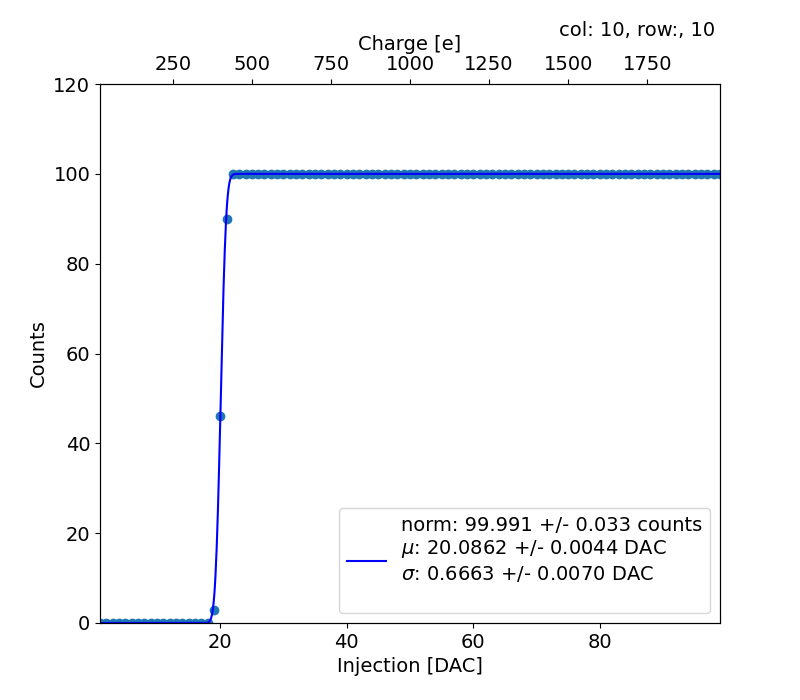
\includegraphics[width=.6\linewidth]{figures/charaterization/scurve.png}
            \caption{S curve for pixel (10, 10) of the PMOS flavor}
            \label{fig:scurve}
        \end{figure}   
        
    
        \begin{figure}[h!]
                -\begin{subfigure}{.5\textwidth}
                \centering
                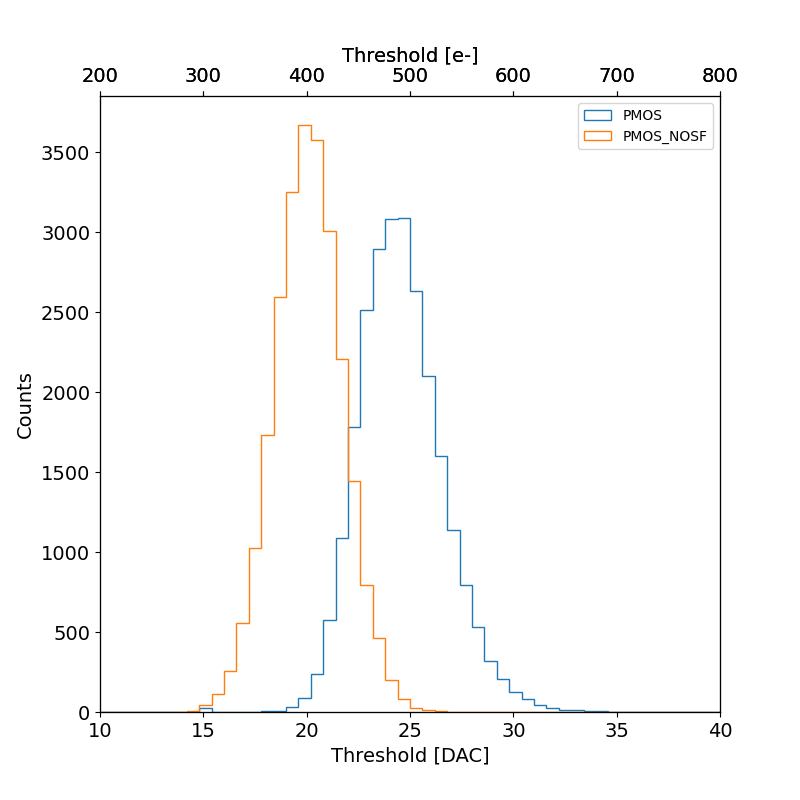
\includegraphics[width=.99\linewidth]{figures/charaterization/threshold_histogram.png}
                \caption{}
                \label{fig:}
                \end{subfigure}
                \begin{subfigure}{.5\textwidth}
                \centering
                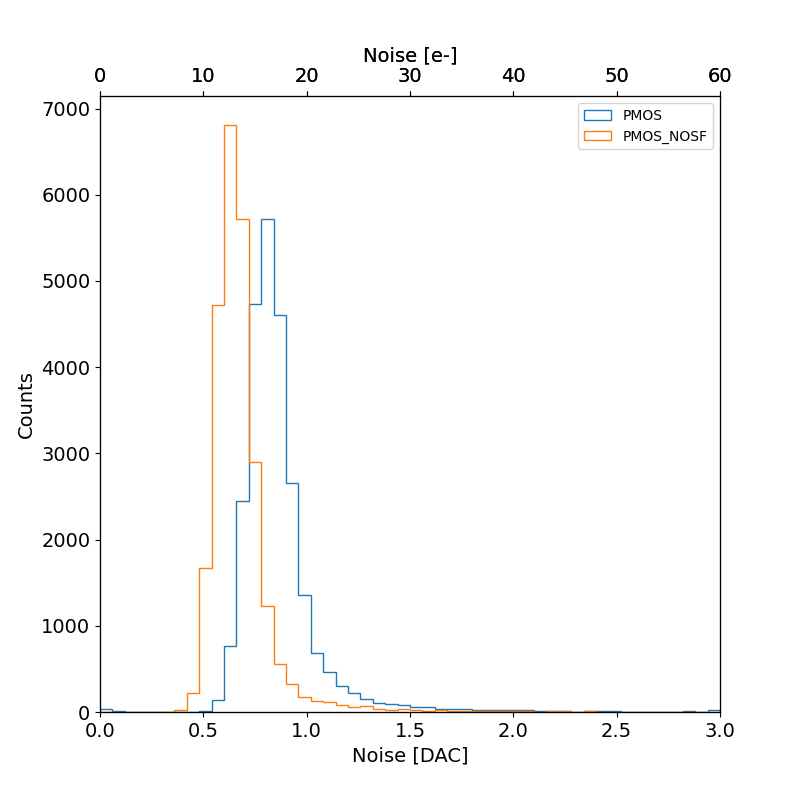
\includegraphics[width=.99\linewidth]{figures/charaterization/noise_histogram.png}
                \caption{}
                \label{fig:}
                \end{subfigure}
        \end{figure}            
           
    
    
        \begin{table}
                \begin{center}
                \begin{tabular}{| c | c | c |}
                \hline
                 & DAC units & electrons \\
                \hline
                \hline
                Threshold        & 24.529 $\pm$ 0.049 & \\
                                 &u: 24.433 $\pm$ 0.049 & \\ 
                                 &d: 24.623 $\pm$ 0.051 &    \\      
                Threshold dispersion & 1.848 $\pm$ 0.033 &\\
                                 &u: 1.867 $\pm$ 0.034 & \\ 
                                 &d: 1.825 $\pm$ 0.035 &    \\ 
                Noise            & 0.8222 $\pm$ 0.0043 & \\
                                 &u: 0.8225 $\pm$ 0.0045 & \\ 
                                 &d: 0.8221 $\pm$ 0.0043 &    \\      
                Noise dispersion & 0.0975 $\pm$ 0.0030 &\\
                                 &u: 0.0968 $\pm$ 0.0031 & \\ 
                                 &d: 0.0970 $\pm$ 0.0030 &    \\ 
                \hline
                \end{tabular}
                \caption{Flavor PMOS}
                \label{tab:}
                \end{center}
        \end{table}        
            
             
                   
        

    \subsection{Calibration of the ToT}    
        %python3 -i acquisition_Fe55/fit_tot_single_pixel.py -f acquisition_Fe55/source_PMOSS/ per fare il fit    
        %python3 -i acquisition_Fe55/plot_tot_single_pixel.py -f acquisition_Fe55/source_PMOSS/ -fl 'gauss_line' per fare il plot di single pixel

        \begin{figure}[h!]
            \begin{subfigure}{.5\textwidth}
            \centering
            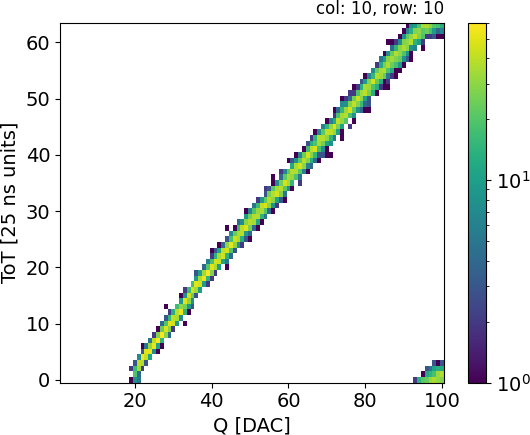
\includegraphics[width=.98\linewidth]{figures/charaterization/ToT_rollover.png}
            \caption{ToT rollover for pixel (10,10). The ToT is in range 0-64 since it is represented by 6 bit.}
            \label{fig:}
            \end{subfigure}
            \begin{subfigure}{.5\textwidth}
            \centering
            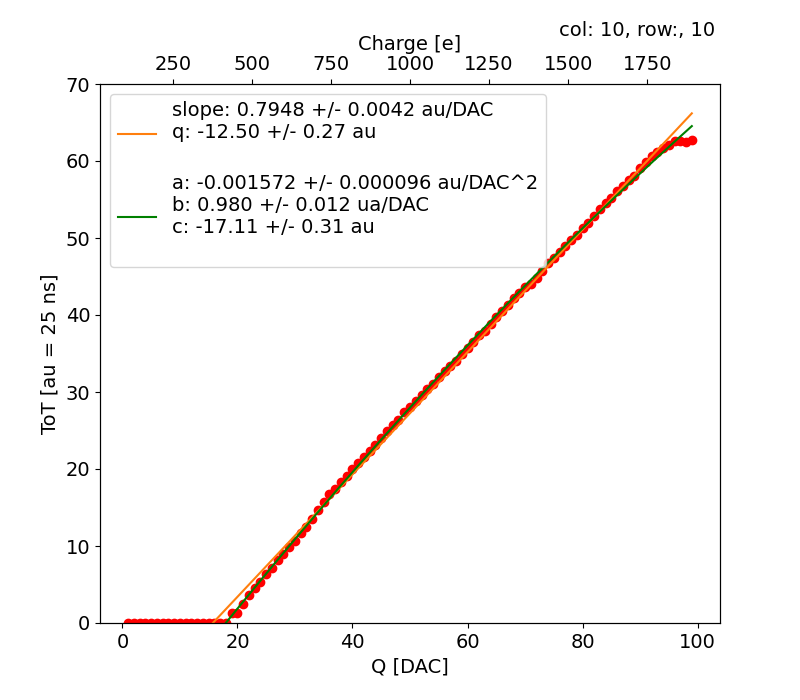
\includegraphics[width=.98\linewidth]{figures/charaterization/ToT_injection.png}
            \caption{}
            \label{fig:}
            \end{subfigure}
        \end{figure}    

        \begin{figure}[h!]
            \begin{subfigure}{.5\textwidth}
            \centering
            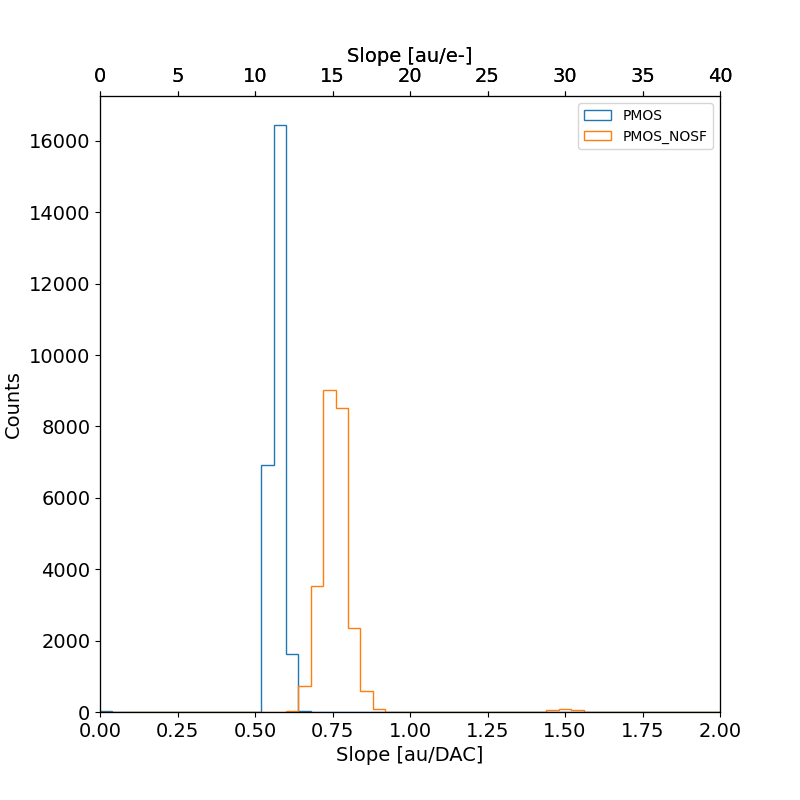
\includegraphics[width=.98\linewidth]{figures/charaterization/slope_histogram.png}
            \caption{}
            \label{fig:}
            \end{subfigure}
            \begin{subfigure}{.5\textwidth}
            \centering
            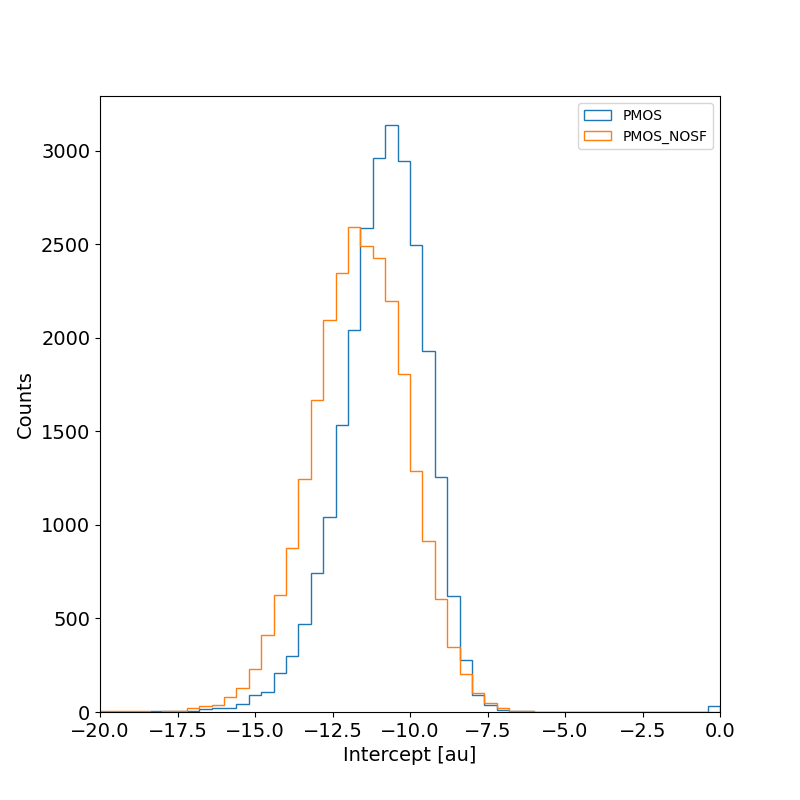
\includegraphics[width=.98\linewidth]{figures/charaterization/intercept_histogram.png}
            \caption{}
            \label{fig:}
            \end{subfigure}
        \end{figure} 

        \begin{table}
            \begin{center}
            \begin{tabular}{| c  c | c | c |c |}
            \hline
             & PMOS & & HV \\
            \hline
            \hline
            Slope [au/DAC] & 0.57145 $\pm$ 0.00025 \\
            Slope dispersion [au/DAC] &  0.01685 $\pm$ 0.00016\\
            Intercept [au] & -10.824 $\pm$ 0.019 \\
            Intercept dispersion [au] & 1.225 $\pm$ 0.013\\
            \hline
            \end{tabular}
            \caption{}
            \label{tab:}
            \end{center}
        \end{table}        

        \subsubsection{Absolute calibration}
        %python3 -i acquisition_Fe55/fit_tot_single_pixel.py -f acquisition_Fe55/source_PMOSS/Fe_acquisitions_6V/ per fare i fit. Attenzione che prende i file degli istogrammi npz già
        \begin{equation}
            f(x, m, q, N, \mu, \sigma) = m\,x + q + \frac{N}{\sigma \sqrt{2\pi}} e^{-\frac{1}{2}(\frac{(x-\mu)}{\sigma})^2}
        \end{equation}   
         
        \begin{figure}[h!]
            \begin{subfigure}{.5\textwidth}
            \centering
            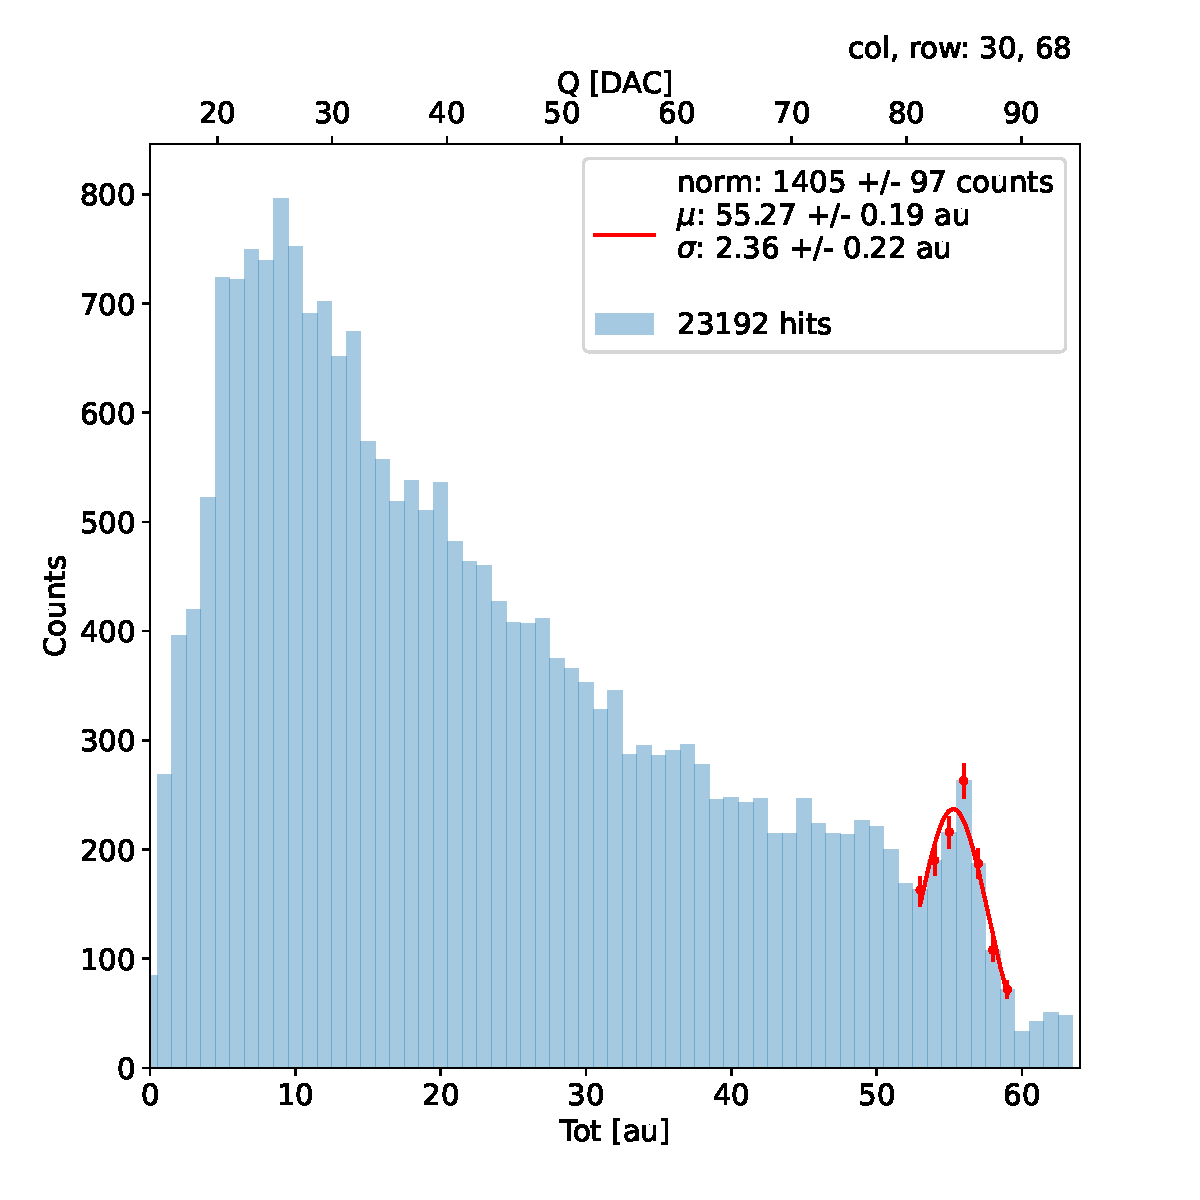
\includegraphics[width=.99\linewidth]{figures/charaterization/fit_gauss_r69.pdf}
            \label{fig:}
            \end{subfigure}
            \begin{subfigure}{.5\textwidth}
            \centering
            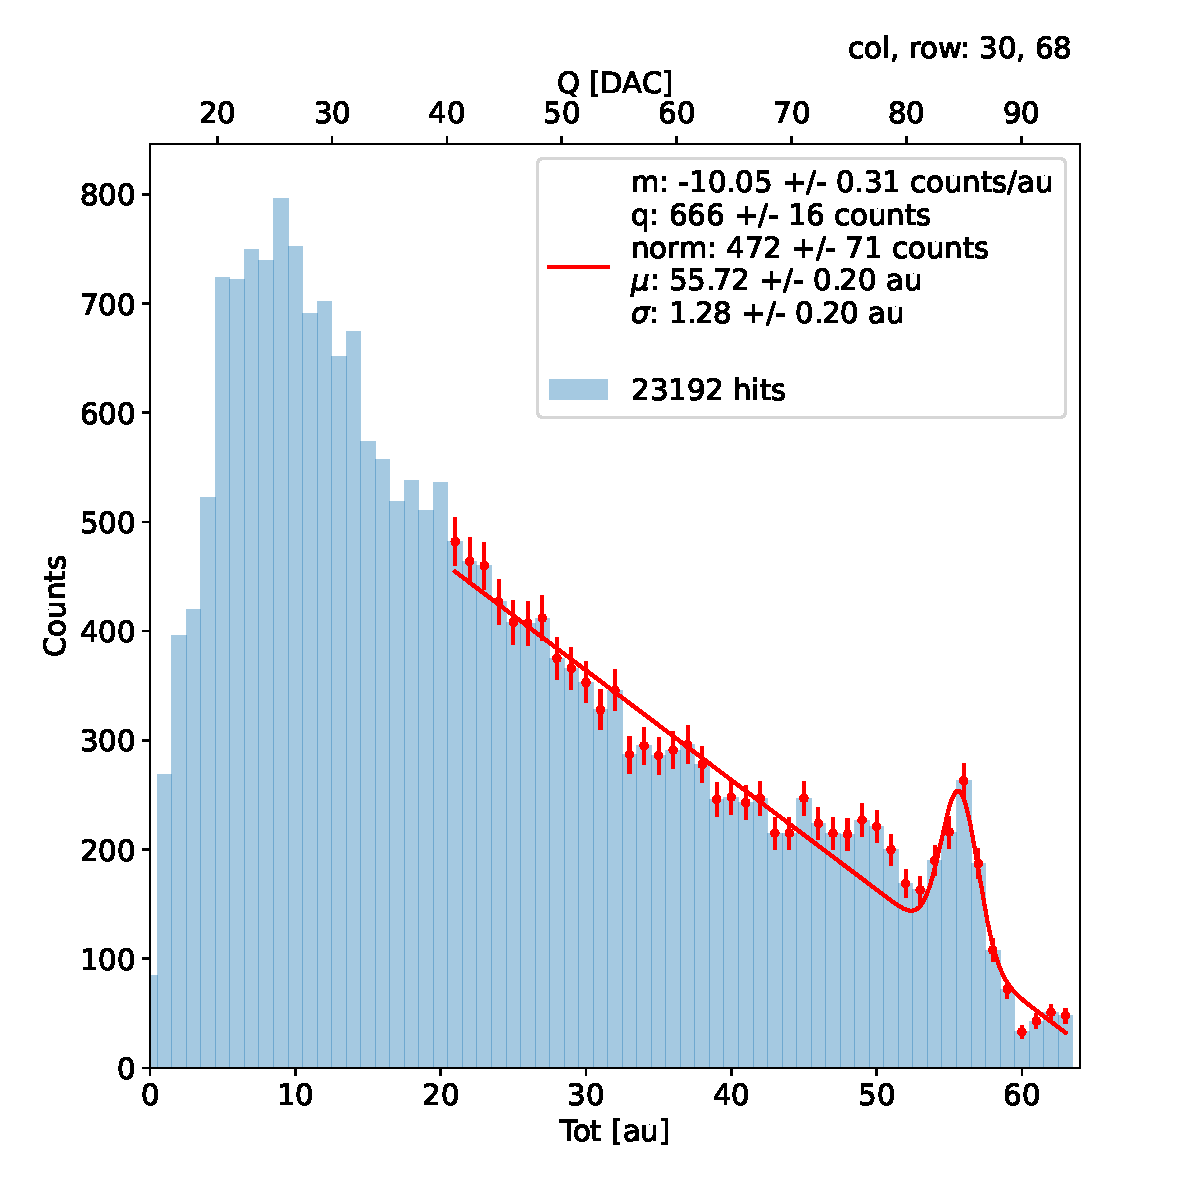
\includegraphics[width=.99\linewidth]{figures/charaterization/fit_line_gauss_r69.pdf}
            \label{fig:}
            \end{subfigure}
            \caption{due pixel per far vedere la differenza tra i fit}
        \end{figure}            

        \begin{figure}[h!]
            \begin{subfigure}{.5\textwidth}
            \centering
            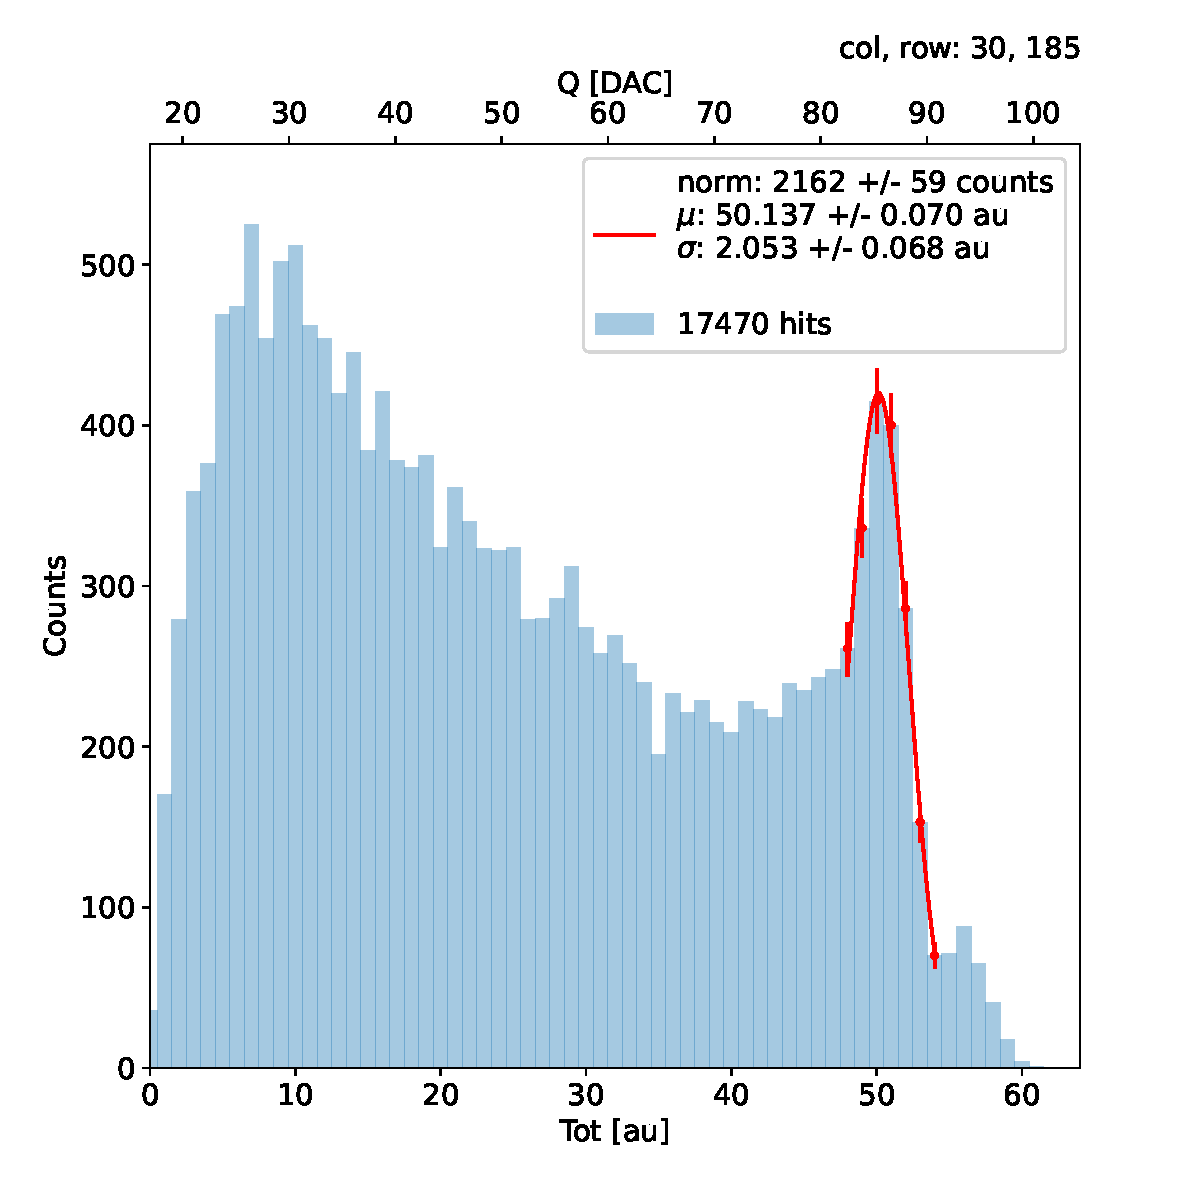
\includegraphics[width=.99\linewidth]{figures/charaterization/fit_gauss_r185.pdf}
            \label{fig:}
            \end{subfigure}
            \begin{subfigure}{.5\textwidth}
            \centering
            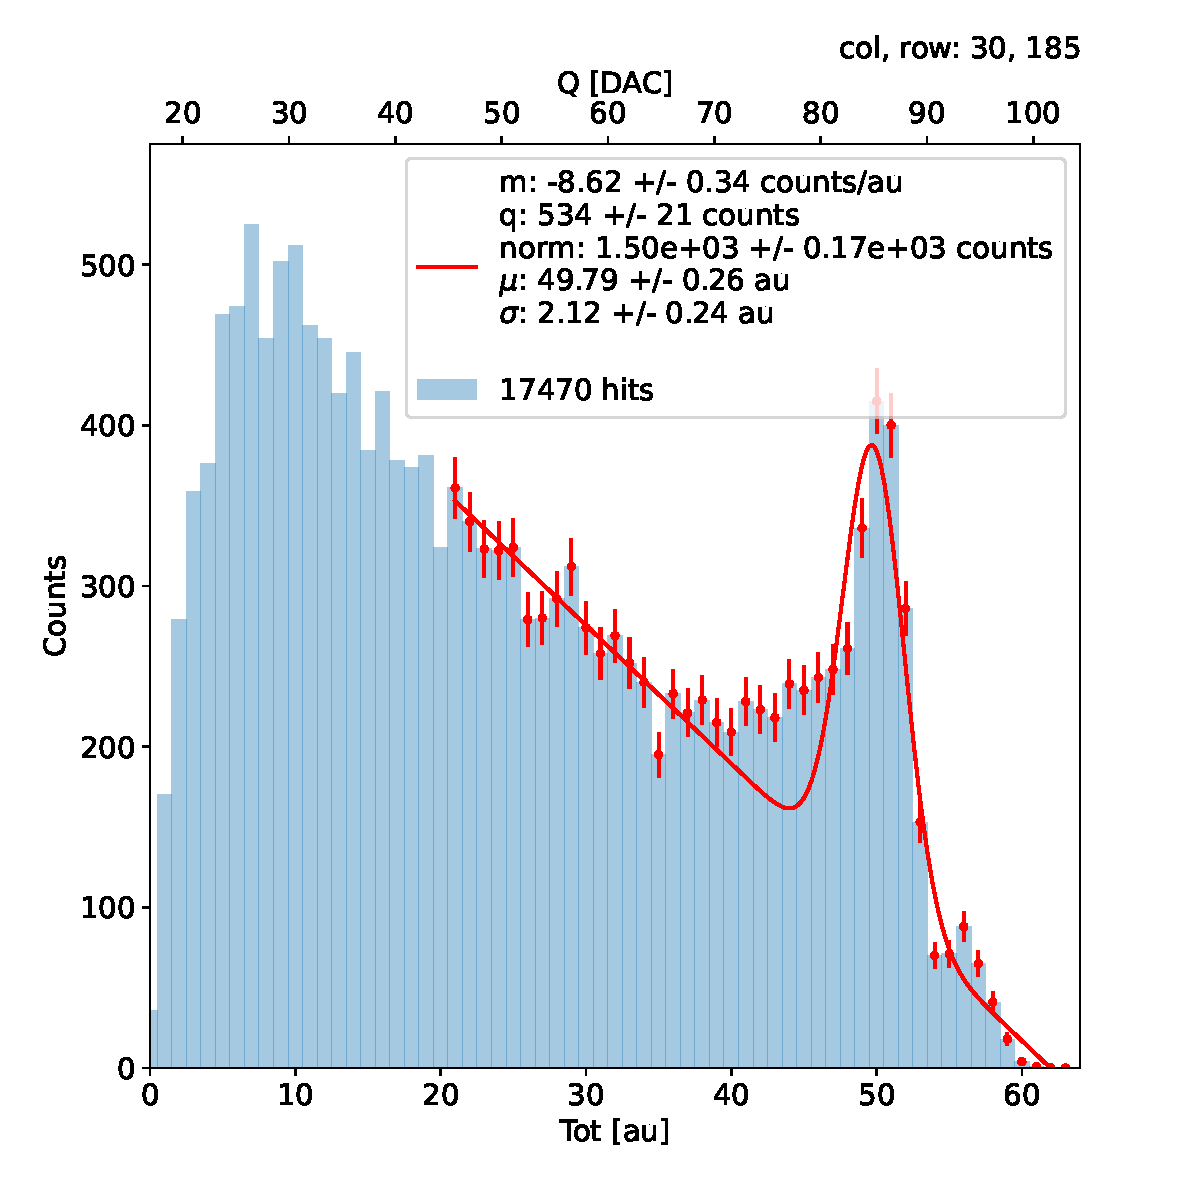
\includegraphics[width=.99\linewidth]{figures/charaterization/fit_line_gauss_r185.pdf}
            \label{fig:}
            \end{subfigure}
            \caption{due pixel per far vedere la differenza tra i fit}
        \end{figure}    
         Mappa dei parametri del fit sulla matrice (media e sigma)
        
         \section{Fe vs bias}
         \begin{itemize}
             \item rate vs bias 
             \item posizione del picco del ferro vs bias    
             \item eventi sotto il picco vs eventi nella coda
         \end{itemize}
     
     
     \section{Measurements with radioactive sources}
         \red{CI metterei i plot con ferro, stronzio e cosmici}
         %python3 -i acquisition_Fe55/find_cluster.py -d acquisition_Fe55/source_PMOSS/noise_acquisitions_6V -> per cluster dimension e spettro del noise
         %python3 -i acquisition_Fe55/hit_map.py -f acquisition_Fe55/source_PMOSS/2022-04-07/2022-04-07_10-10-01_acq.h5 -> per le hit map, comprese qualche hitmap dei cluster
         %python3 -i acquisition_Fe55/Sr90_spectrum.py -d acquisition_Fe55/source_PMOSS/noise_acquisitions_6V/ -> per fare i plot dello stronzio
         ToT con doppia scala (calibrata in elettroni e non in ToT)
         hit per cluster
         dimensione cluster
         hit map di un paio di tracce?
        \subsection{Dead time measurements}
        The hit loss is due to analog and digital pile up: the first one occurs when a new hit arrives during the pre-amplifier response, the second instead, which is the more relevant contribution with high rate, while the information of the previous hit has not yet been transferred to the periphery.  
        As only one hit at a time can be stored on the pixel's RAM, until the data have completed the path to get out, the pixel is paralyzed and the dead time $\tau$ almost corresponds with the time needed to trasmit the data-packets off-chip.
        Since the exportation of data from pixel to the EoC occurs via a 21-bits data bus, only one clock cycle is need to transfer the data to the end of column and the dead time bottleneck is given by the bandwidth of the serializer at the EoC. In our setup the serializer operates at 40 MHz, thus to transmit a data packet (27-bit considering the addition at the EoC) at least \SI{675}{ns} are needed. 
        For what we have said so far, the R/O is completely sequential and therefore is expected a linear dependence of the reading time on the number of pixels to read:
        \begin{equation}
            \tau =\, 25\: \unit{ns}\, \times\, (\alpha\, N +\, \beta)
            \label{eq:reading_time}
        \end{equation}
        where $\alpha$ and $\beta$ are parameters dependent on the readout chain setting. 
        
        To measure and test the linearity of the reading time with the number of pixels firing, I have used the injection mode available on the chip. 
        Indeed, the injection mode allows fixing not only the amplitude of the pulse, which corresponds to the charge in DAC units, but also the period and the width.
        I have injected a fix number of pulses (100) and looked for the rate when the efficiency decreases. 
        Moreover to test that there is no dependece of the digital readout time from the charge of the pulse, I have try to change the amplitude of the pulse injected, but the parameters found were consistent with the default configuration ones.

        \red{Al posto degli esempi con 5 e 10 pixels metterei un esempio dell'efficienza vs il periodo quando leggo un singolo pixel. Una cosa che volevo fare era anche provare a fittare la slope con cui l'efficienza scende: se la slope è uguale per tutti il readout diventa completamente predittivo. }
        \begin{figure}[h!]
            \begin{subfigure}{.5\textwidth}
            \centering
            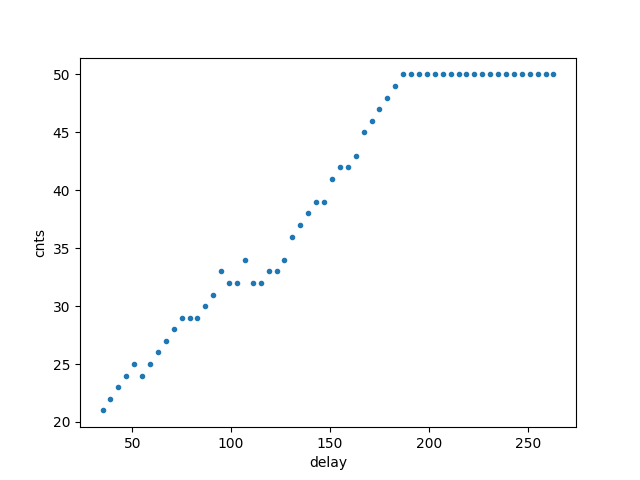
\includegraphics[width=.98\linewidth]{figures/charaterization/efficiency_5pixels.png}
            \caption{\red{efficiency vs DELAY 5 pixels}}
            \label{fig:}
            \end{subfigure}
            \begin{subfigure}{.5\textwidth}
            \centering
            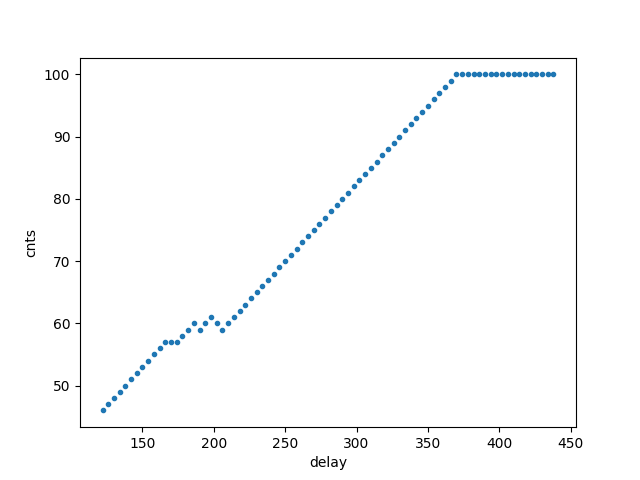
\includegraphics[width=.98\linewidth]{figures/charaterization/efficiency_10pixels.png}
            \caption{\red{efficiency vs DELAY per 10pixels}}
            \label{fig:}
            \end{subfigure}
        \end{figure}
        
        While the single pixel reading time and the dead time do not depend on the position on the pixel matrix and are equal to \red{106 (46+60)} clock counts within 1 clock count, on the other hand the $\tau$ depends on the pixel position on the matrix when more than one pixel are firing. 
        In particular the priority chain goes from row 224 to row 0, and from col 0 to 112, that means the last pixels to be read is the one on le bottom right corner of the matrix. 

        In figure \ref{fig:dead_time} is reported the reading time versus the number of pixels injected; the R/O parameters that control the reading time and their default values are reported on table \ref{tab:tab:R/O_param}.
        \begin{table}
            \begin{center}
            \begin{tabular}{|c | c | c |}
            \hline
            Parameter & Value [\si{DAC}] & Value [\si{\us}]\\
            \hline
            \hline
            START\_FREEZE & 64 & 1.6\\
            STOP\_FREEZE & 100 & 2.5\\
            START\_READ & 66 & 1.65\\
            STOP\_READ & 68 & 1.7\\
            \hline
            \end{tabular}
            \caption{Default configuation of the R/O parameters}
            \label{tab:R/O_param}
            \end{center}
        \end{table}

        The factor $\alpha$, referring to eq. \ref{eq:reading_time} is proportional to the difference (STOP\_FREEZE - START\_READ), while the offset $\beta$ lies between 5 and 15 clock counts.
        Since through the injection a random hit rate on the matrix can't be simulated, as the coordinates of the pixels to inject must be specified, for convenience I used the pixels on the same column/row. No difference in the $\alpha$ and $\beta$ coefficients has been observed between the two case. 
        \begin{figure}[h!]
            \centering
            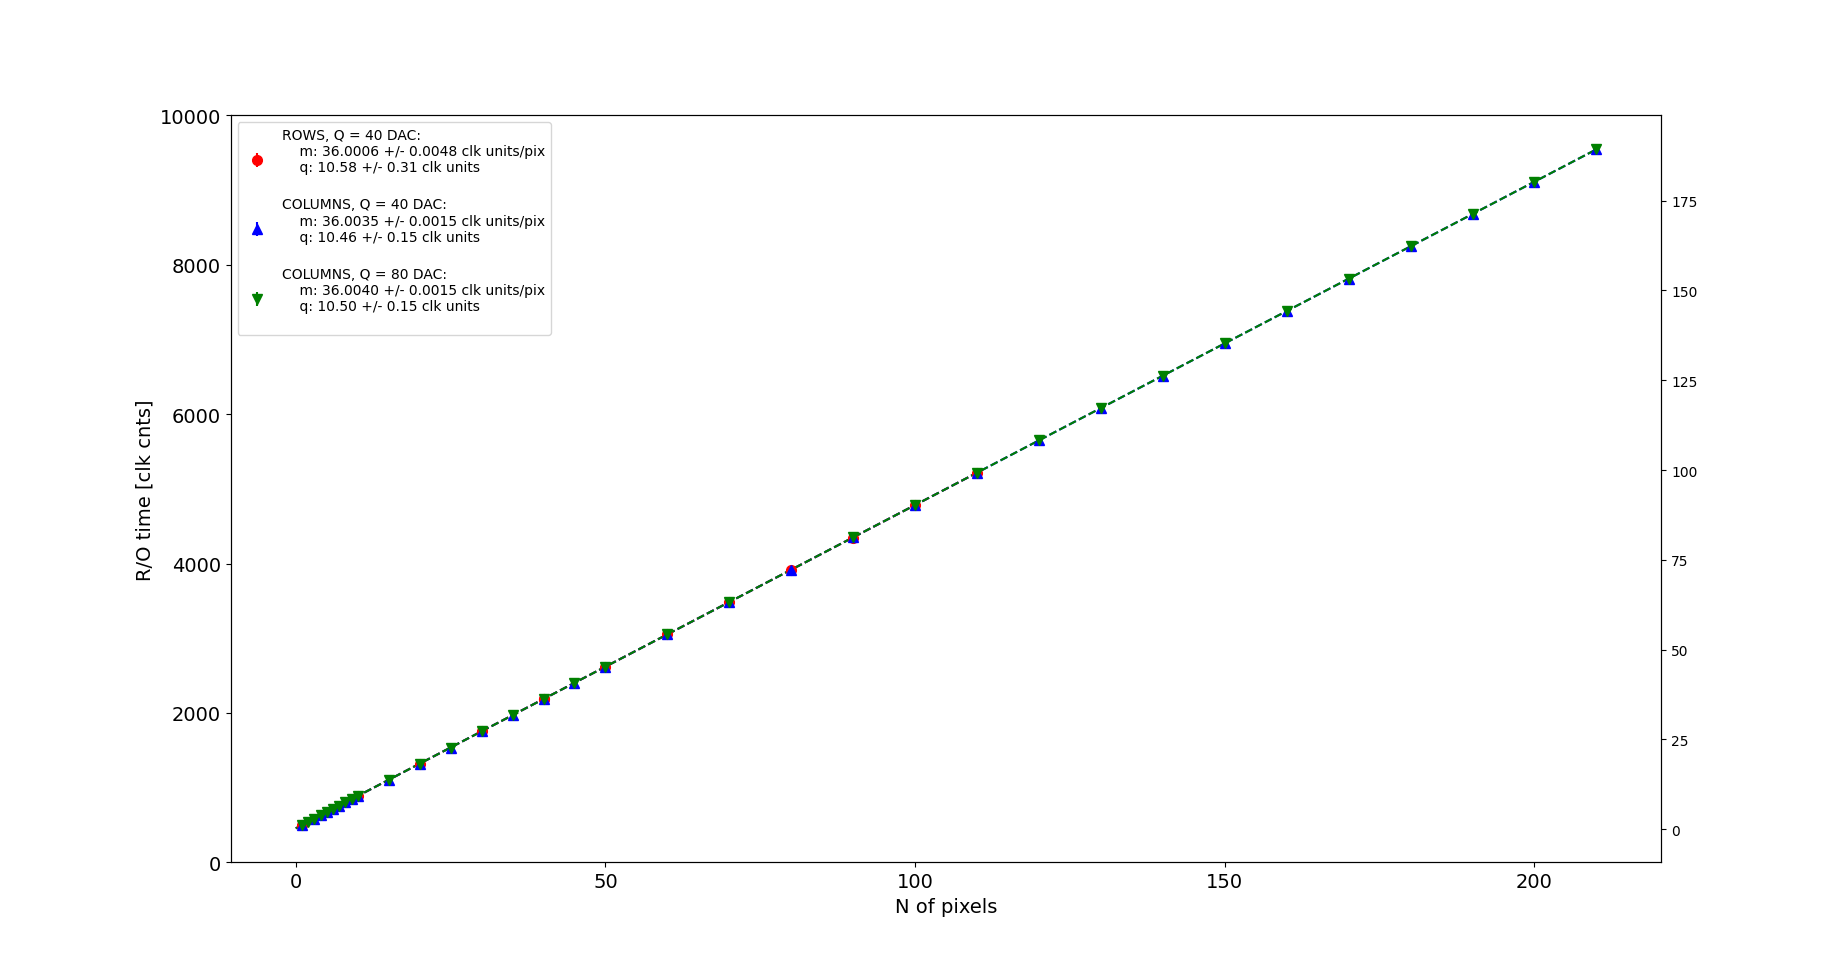
\includegraphics[width=.9\linewidth]{figures/charaterization/default_line.png}
            \caption{}
            \label{fig:dead_time}
        \end{figure}

        \begin{figure}[h!]
            \centering
            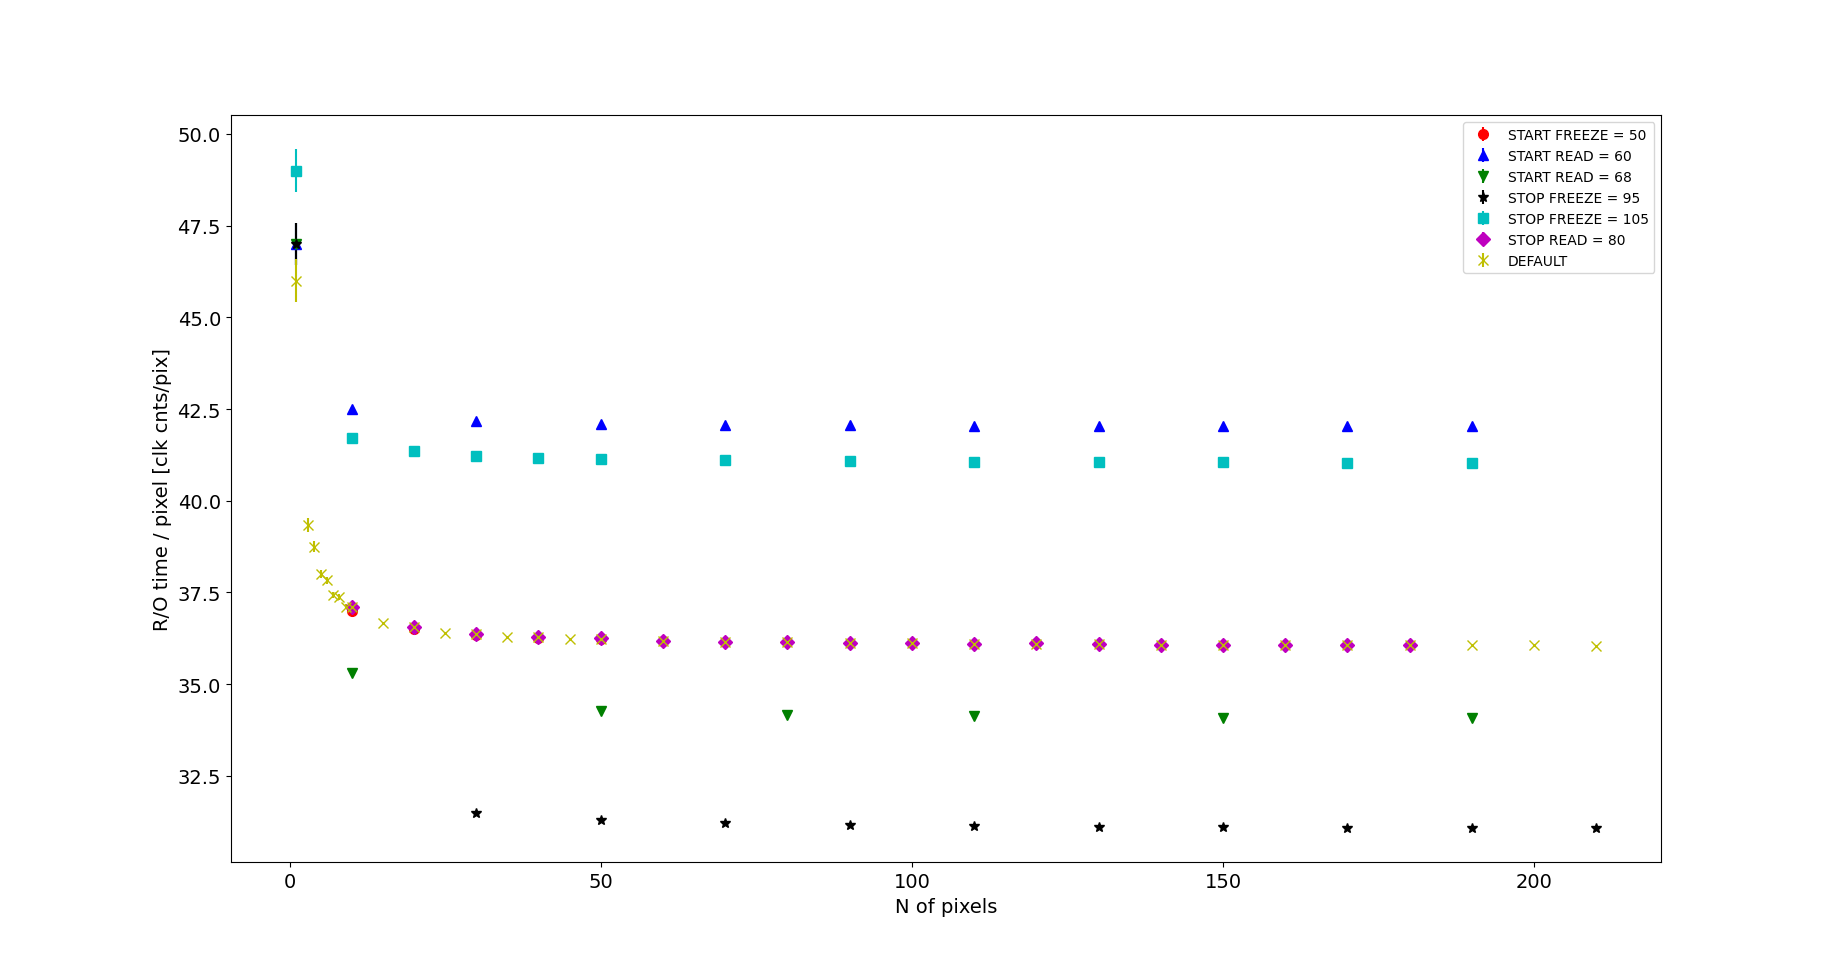
\includegraphics[width=.9\linewidth]{figures/charaterization/parameters_points.png}
            \caption{}
            \label{fig:dead_time}
        \end{figure}        

        \red{Ci sarebbe da spiegare perchè i parametri che usiamo noi come default non sono quelli che minimizzano il tempo di lettura. La spiegazione è che "Abbiamo copiato i valori dal repositorio di quelli di Bonn". Un'altra domanda potrebbe essere: come mai non ho esplorato una zona più vasta per i parametri del R/O. Cambiando molto i parametri del R/O la lettura non funzionava per niente: ad esempio CONF\_STOP\_FREEZE non può essere impostato nè sopra 105 nè sotto 95}



\section{ARCADIA-MD1 characterization}
